\documentclass[margin=5mm, tikz]{standalone}
\usepackage[utf8x]{inputenc}
\usepackage{tikz}
\usepackage{siunitx}
\usepackage{physics}
\begin{document}
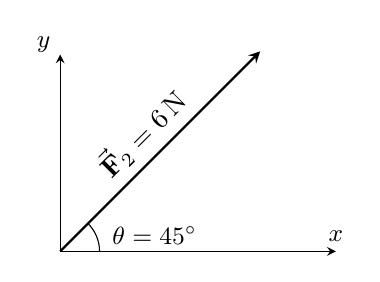
\begin{tikzpicture}
    
    \draw [-stealth] (0, 0) -- (3.5, 0) node [above, pos=1] {\small{$x$}};
    \draw [-stealth] (0, 0) -- (0, 2.5) node [left, pos=1.05] {\small{$y$}};

    \draw [-stealth, thick] (0, 0) -- (2.54, 2.54) node [above, midway, rotate=45] {$\va{F}_{2} = \SI{6}{\newton}$};
    \draw (0.5, 0) arc(0:45:0.5);
    \node at (1.2, 0.2) {\small{$\theta = \ang{45}$}};
    \draw (0, 0) -- (2.5, 0); 

    % \draw [-stealth, thick] (2, 0) -- (2, 2) node [right, midway] {$A_{y}$}; 
    % \draw [-stealth, thick] (0, 0) -- (2, 0) node [below, midway] {$A_{x}$};

    % \draw (1.6, 0) -- (1.6, 0.2) -- (2, 0.2);
    
\end{tikzpicture}
\end{document}